\documentclass[fontsize=14pt,a4paper]{scrartcl}
\usepackage{graphicx}
\usepackage{float}
\usepackage[T1]{fontenc}
\usepackage[utf8]{inputenc}
\include{prologue}
\usepackage{listings}
\usepackage{enumitem}
\usepackage{amssymb}
\usepackage{amsmath}

\begin{document}
\title{REI105M\\Forritun Ofurtölva\\Assignment 1}
\author{Helga Lilja Jónsdóttir and Þór Tómasarson}
\maketitle
\sloppy

\setlength\parindent{24pt}

\begin{enumerate}
    \item
    Understanding the Jötunn cluster environment
    \begin{enumerate}[label*=\arabic*.]
    \item
    \textit{Hello world job script.}
    The scheduler sbatch gets notified of a new task via the command:
    \begin{lstlisting}
    $ sbatch submit-helloworld.sh
    \end{lstlisting}
    The submit-helloworld.sh bash script is structured according to the sbatch requirement and specifies, what program should be executed, how many nodes are required and what modules should be loaded.
    \begin{figure}[H]
        \centering
        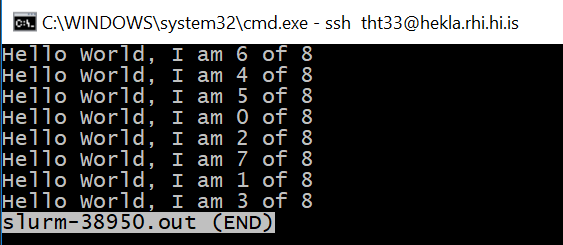
\includegraphics{Images/HelloWorld-8}
        \caption{\textbf{Hello World} program on 8 nodes}
    \end{figure}
    \begin{figure}[H]
        \centering
        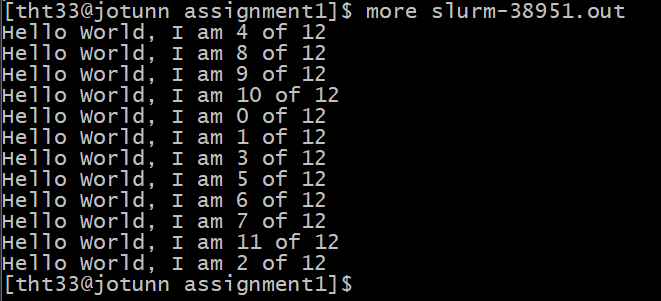
\includegraphics[scale=0.8]{Images/HelloWorld-12}
        \caption{\textbf{Hello World} program on 12 nodes}
    \end{figure}

    \item
    \textit{Pingpong program sending ``12345''.}
    
    The ping pong program needs to be scheduled on two nodes. The program initializes the MPI environment and gets assigned it's rank id $0$ or $1$ as well getting notified of the number of nodes running.

    Then depending on whether the node running the program is rank $0$ or $1$ it starts by either sending the message (ping) $int outmsg=12345$, if rank $0$ and if rank $1$ then it goes straight into waiting for a message with MPI\_Recv. After successful message transfer node $1$ proceeds to sending the same message back (pong) and node $0$ proceeds to waiting for the message. Once the message has been successfully transfered both nodes proceed to printing there debug message and then exit after MPI\_Finilize call.
    \begin{figure}[H]
        \centering
        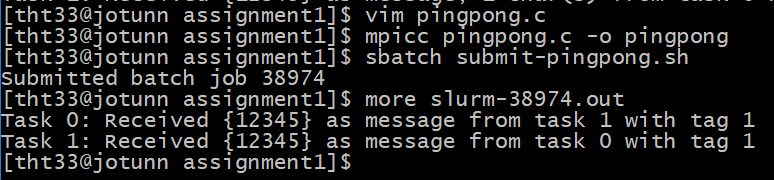
\includegraphics[scale=0.8]{Images/Pingpong}
        \caption{Output from execution of the \textbf{ping pong} program}
    \end{figure}

    \item
    \textit{Scatter and gather program}
    The scatter gather program was structured so that node of rank 0 controls the data distribution. On startup an array is constructed $array = [0, 1, 2, ..., (N * 4) - 1]$ where N is the number of nodes. Then each node receives an array chunk of 4 elements with the scatter command. The node then computes the sum of it’s elements and reports them back with via the gather command. The rank 0 node computes the sum of the gathered sums and prints the result to the standard output.
    \begin{figure}[H]
        \centering
        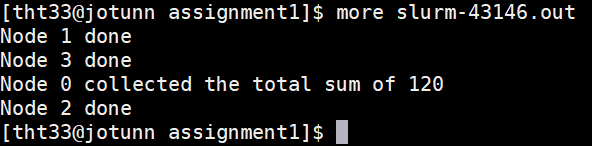
\includegraphics[scale=0.8]{Images/ScatterGather}
        \caption{Output from execution of the \textbf{scatter gather} program with 4 nodes}
    \end{figure}

    \item
    \textit{Parallel pizza MPI program}
    % TODO: Upload the code to UGLA as a zipped file allong with the job script.
    % Brod cast | 2 x communicatiors | MPI_Barrier to block them from going to early

    \end{enumerate}
\end{enumerate}

\end{document}
